\newpage
\section{Ciclo di vita}
Il modello di ciclo di vita adottato per Premi è il \textbf{modello incrementale}, per le sue proprietà qui elencate:

\begin{itemize}
	\item suddivide il prodotto finale in un numero di componenti, ognuno dei quali viene costruito (e verificato) separatamente per ordine di importanza. Questo permette di verificare con più precisione che tutti requisiti vengano soddisfatti perchè sono facilmente associabili ad uno o più componenti. È importante notare che la creazione di un sito web, suddiviso in pagine, gerarchie e funzionalità si presta naturalmente ad una costruzione di tipo incrementale;
	\item Sposta le attività principali di sviluppo, analisi e progettazione architetturale ad alto livello all'inizio del ciclo garantendo una codifica allo stesso tempo controllata e snella. Anche gli incrementi vengono pianificati e questo aiuta a stimare costi e tempi di produzione;
	\item Favorisce la creazione di prototipi che consentono una maggiore visione di insieme e migliorano il dialogo con il committente;
	\item Ogni incremento riduce il rischio di fallimento perchè consolida la sezione coinvolta (ogni incremento produce una base da considerarsi stabile);
	\item Le risorse umane possono essere distribuite a rotazione su di un numero limitato di attività, per brevi periodi di tempo, assumendo ruoli diversi. Questo è in linea con la richiesta dei docenti di far ricoprire più ruoli ai componenti del gruppo, garantendo però assenza di conflitto di interessi tra i ruoli assunti.
\end{itemize}	

\section{Scadenze}
Qui vengono presentate le date di consegna delle revisioni che il gruppo 404NotFound ha deciso di rispettare per lo sviluppo del software:

\begin{itemize}
	\item \textit{Revisione dei Requisiti} (RR): 2015-02-16 \\
	Data di consegna della documentazione: 2015-01-23;
	\item \textit{Revisione di Progetto} (RP): 2015-04-27 \\
	Data di consegna della documentazione: 2015-04-22;
	\item \textit{Revisione di Qualifica} (RQ): 2015-05-29 \\
	Data di consegna della documentazione: 2015-05-24;
	\item \textit{Revisione di Accettazione} (RA): 2015-06-18 \\
	Data di consegna della documentazione: 2015-06-17.
\end{itemize}
\section{Ruoli}

I ruoli previsti per la realizzazione del progetto sono:

\begin{itemize}
	\item \textbf{Responsabile del Progetto:} È il responsabile ultimo, per conto del suo gruppo, dei risultati del progetto.
Elabora ed emana piani e scadenze, approva l'emissione di documenti, coordina le attività del gruppo, si relaziona con il controllo di qualità interno al progetto, redige l'Organigramma e il Piano di Progetto e approva l'Offerta e i relativi allegati.
	\item \textbf{Analista:} È responsabile dell'efficienza e dell'operatività dell'ambiente di sviluppo. 
È responsabile della redazione e attuazione di piani e procedure di Gestione per la Qualità, controlla versioni e configurazioni del prodotto, gestisce l'archivio della documentazione di progetto, collabora alla redazione del Piano di Progetto e redige le Norme di Progetto per conto del \ruoloResponsabile{}.
	\item \textbf{Progettista:} È responsabile delle attività di analisi. 
Redige lo Studio di Fattibilità (documento interno al gruppo) e l'Analisi dei Requisiti.
	\item \textbf{Amministratore:} È responsabile delle attività di progettazione. 
Redige Specifica Tecnica, Definizione di Prodotto e la parte programmatica del Piano di Qualifica.
	\item \textbf{Verificatore:} È responsabile delle attività di codifica miranti alla realizzazione del prodotto e delle componenti di ausilio necessarie per l'esecuzione delle prove di verifica e validazione.
	\item \textbf{Programmatore:} È responsabile delle attività di verifica.
Redige la parte retrospettiva del Piano di Qualifica che illustra l'esito e la completezza delle verifiche e delle prove effettuate secondo il piano.
\end{itemize}

\begin{table}[h]
\begin{center}
\begin{tabular}{|l|l|}
\hline
\textbf{Ruolo} & \textbf{€/ora} \\
\hline
\ruoloResponsabile & 30 \\
\ruoloAnalista & 25 \\
\ruoloProgettista & 22 \\
\ruoloAmministratore & 20 \\
\ruoloVerificatore & 15 \\
\ruoloProgrammatore & 15 \\
\hline
\end{tabular}
\caption{Ruoli previsti e costo per ruolo.}
\end{center}
\end{table}

Anzichè effettuare una ripartizione dei ruoli casuale si è preferito specializzare le Risorse Umane nella stesura di determinati documenti, pur mantenendo una quasi assoluta assenza di conflitto di interessi. Si potrà comunque notare che ogni membro del gruppo assume quasi tutti i ruoli nel corso del progetto, e che attività come la Codifica sono state spartite equamente per non causare sovraccarichi di lavoro nei periodi di sviluppo più intensi. Per ulteriori informazioni consultare le tabelle delle macro-fasi nella sezione sottostante.

\section{Risorse necessarie e disponibili}
Vengono qui riportate le risorse hardware e software necessarie alle attività di verifica, validazione e collaudo del prodotto, tutte già in possesso dal gruppo.

\subsection{Ambiente Desktop}
I seguenti sistemi operativi:
\begin{itemize}
\item Microsoft Windows XP
\item Microsoft Windows 8
\item Linux Ubuntu 14.04
\item Apple MacOs 
\end{itemize}
I seguenti browser:
\begin{itemize}
\item Microsoft Internet Explorer 8
\item Microsoft Internet Explorer 11
\item Apple Safari
\item Mozilla Firefox
\item Google Chrome
\end{itemize}
Le seguenti risoluzioni di monitor:
\begin{itemize}
\item 1024x764
\item 1440x960
\item 1920x1080
\end{itemize}

\subsection{Ambiente Mobile}
I seguenti sistemi operativi:
\begin{itemize}
\item Android
\item iOS
\item Windows Phone 8.1
\end{itemize}

\subsection{Ambiente Server}
I seguenti sistermi operativi:
\begin{itemize}
\item Ubuntu Server 14.04
\end{itemize}



\newpage
\section{Pianificazione delle attività}
Lo sviluppo di Premi, in linea con le scadenze sopra elencate, viene diviso in quattro macro-fasi:

\begin{itemize}
\item \textbf{Analisi} (AN) dal 2014-12-01 al 2015-01-22;
\item \textbf{Progettazione Architetturale} (PA) dal 2015-02-17 al 2015-04-21;
\item \textbf{Progettazione di Dettaglio e Codifica} (PDC) dal 2015-04-22 al 2015-05-23;
\item \textbf{Verifica Finale e Validazione} (VV) dal 2015-05-24 al 2015-06-16.
\end{itemize}

Ogni macro-fase è a sua volta divisa nelle sue attività essenziali, e ogni attività è composta da sotto-attività che ne disciplinano la realizzazione.\\
La durata di ogni attività è stata tracciata con diagrammi di Gantt$_{G}$, disegnati dal software \href{http://www.projectlibre.org/}{ProjectLibre}$_{G}$, dai quali si possono visualizzare le dipendenze e le principali milestone$_{G}$. Per calcolare le ore e i costi di lavoro invece si è preferito utilizzare un foglio elettronico per la facilità con cui si possono ricavare automaticamente le somme totali (attraverso le funzioni) e aggiornare i dati in caso di modifiche future al documento.

\subsection{Responsabile del Progetto}
Per la creazione dei ticket$_{G}$ e delle milestone$_{G}$, per la rendicontazione e il controllo dei rischi è stato scelto a rotazione un componente del gruppo per ogni macro-fase.
Egli assumerà il ruolo di \ruoloResponsabile{} e svolgerà questo compito durante le ore a lui già assegnate per le altre attività.

\newpage
\subsection{Analisi}
\textbf{Periodo:} dal 1-12-2014 al 22-01-2015 \\
\textbf{Responsabile:} \VeFe \\
La macro-fase di Analisi inizia dalla formazione del gruppo e prosegue fino alla consegna della documentazione per la Revisione dei Requisiti. \\
I ruoli coinvolti sono quelli del \ruoloResponsabile{}, \ruoloAmministratore{}, \ruoloVerificatore{} e \ruoloAnalista{}, mentre le attività principali sono la stesura e la verifica dei seguenti documenti:

\begin{itemize}
\item \textbf{Studio di fattibilità:} in questo documento vengono studiate le tecnologie interessate e la fattibilità dei Capitolati per stabilire quale affrontare. Sulla scelta pesa molto anche l'interesse dei vari membri del gruppo ai temi proposti;
\item \textbf{Norme di Progetto:} emanate dall'\ruoloAmministratore{}, queste norme disciplinano tutte le attività del gruppo in ogni fase del Ciclo di Vita del software;
\item \textbf{Analisi dei Requisiti:} qui vengono descritti in modo dettagliato i requisiti emersi dal Capitolato e dal successivo incontro con il proponente. Ogni requisito aiuta a delineare le funzionalità del prodotto finale;
\item \textbf{Piano di Progetto:} la stesura di questo documento è compito del \ruoloResponsabile{} e punta a pianificare le attività e a distribuirle nell'arco di tempo stabilito dal gruppo calcolandone i costi totali. Vengono inoltre studiati i possibili rischi a cui il progetto va incontro e vengono suggerite le strategie per affrontarli;
\item \textbf{Piano di Qualifica:} delinea la strategia generale di Verifica e Validazione;
\item \textbf{Glossario:} questo documento contiene le definizioni dei termini e degli acronimi presenti negli altri documenti e ne facilita la compresione. Viene scritto in modo incrementale da tutti i redattori;
\item \textbf{Lettera di Presentazione:} ha il compito di presentare il gruppo al committente e rende ufficiale l'offerta di prendersi in carico il progetto.
\end{itemize}

\newpage
\subsubsection{diagramma di Gantt}

\begin{figure}[h]
\begin{center}
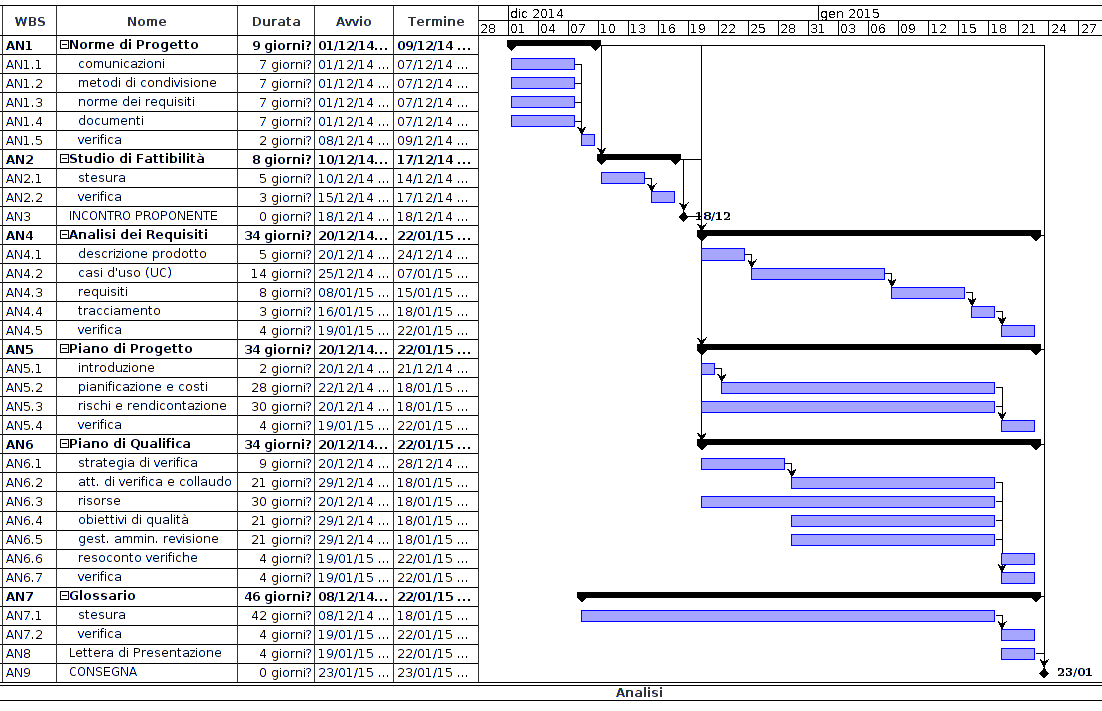
\includegraphics[width=\textwidth, height=\textheight, keepaspectratio]{img/analisi-gantt.png}
\caption{Diagramma di Gantt delle attività della macro-fase di Analisi.}
\end{center}
\end{figure}
\clearpage

\newpage
\subsubsection{tabella persone/ore/attività}

\begin{figure}[h]
\begin{center}
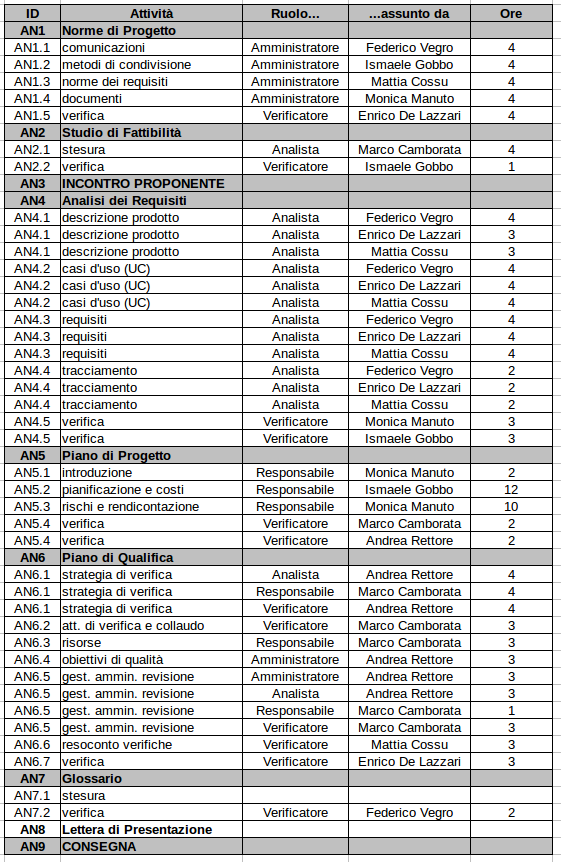
\includegraphics[scale=0.50]{img/analisi-attivita.png}
\caption{Tabella persone/ore/attività della macro-fase di Analisi.}
\end{center}
\end{figure}
\clearpage

\subsubsection{tabella persone/ore/costi}

\begin{figure}[h]
\begin{center}
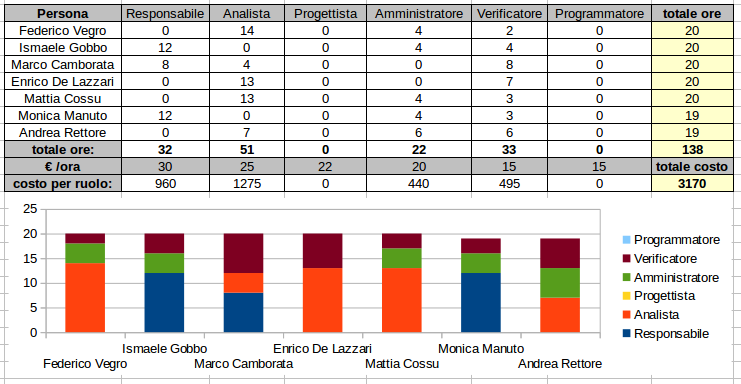
\includegraphics[scale=0.50]{img/analisi-personeorecosti.png}
\caption{Tabella persone/ore/costi della macro-fase di Analisi.}
\end{center}
\end{figure}

\newpage
\subsection{Progettazione Architetturale}
\textbf{Periodo:} dal 17-02-2015 al 21-04-2015 \\
\textbf{Responsabile:} \GoIs \\
La macro-fase di Progettazione Architetturale inizia dalla Revisione dei Requisiti e prosegue fino alla consegna della documentazione per la Revisione di Progetto. \\
I ruoli coinvolti sono quelli del \ruoloResponsabile{}, \ruoloAmministratore{}, \ruoloAnalista{}, \ruoloProgettista{} e \ruoloVerificatore{}, mentre le attività principali sono la stesura e la verifica dei seguenti documenti:

\begin{itemize}
\item \textbf{correzione}, se necessaria, dei documenti usciti dalla precedente fase (la Revisione dei Requisiti potrebbe imporre delle modifiche ad alcune sezioni);
\item \textbf{Specifica Tecnica:} ha lo scopo di definire l'architettura del prodotto finale,  attraverso lo studio dei componenti e l'esposizione dei Design Pattern utilizzati. Ogni componente viene associato ad uno o più requisiti;
\item \textbf{incremento e verifica} dei documenti usciti dalla precendente macro-fase.
\end{itemize}

\newpage
\subsubsection{diagramma di Gantt}

\begin{figure}[h]
\begin{center}
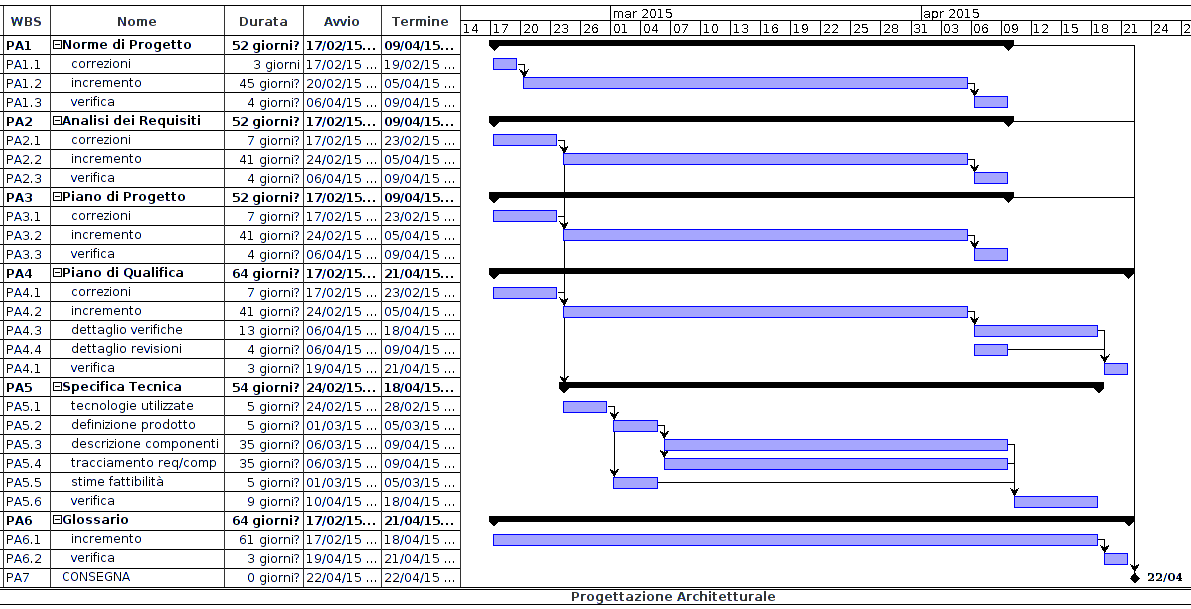
\includegraphics[width=\textwidth, height=\textheight, keepaspectratio]{img/progarc-gantt.png}
\caption{Diagramma di Gantt delle attività della macro-fase di Progettazione Architetturale.}
\end{center}
\end{figure}
\clearpage

\newpage
\subsubsection{tabella persone/ore/attività}

\begin{figure}[h]
\begin{center}
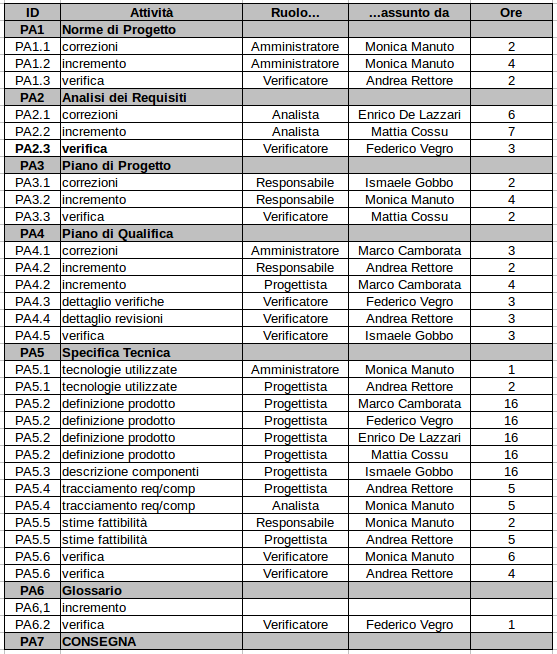
\includegraphics[scale=0.50]{img/progarc-attivita.png}
\caption{Tabella persone/ore/attività della macro-fase di Progettazione Architetturale.}
\end{center}
\end{figure}
\clearpage

\subsubsection{tabella persone/ore/costi}

\begin{figure}[h]
\begin{center}
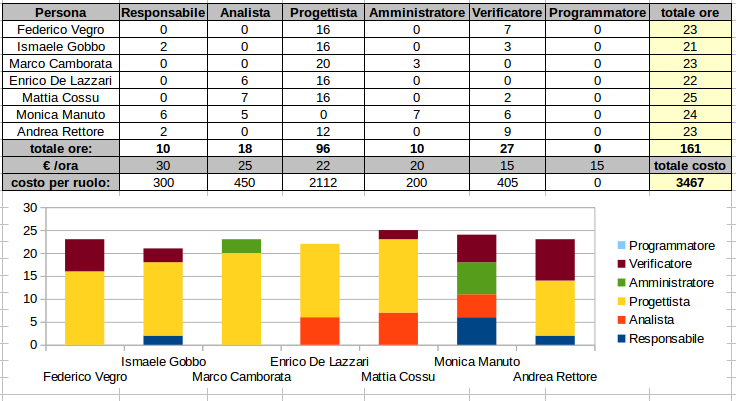
\includegraphics[scale=0.50]{img/progarc-personeorecosti.png}
\caption{Tabella persone/ore/costi della macro-fase di Progettazione Architetturale.}
\end{center}
\end{figure}

\newpage
\subsection{Progettazione di Dettaglio e Codifica}
\textbf{Periodo:} dal 22-04-2015 al 23-05-2015 \\
\textbf{Responsabile:} \CoMa \\
La macro-fase di Progettazione Architetturale inizia dalla Revisione di Progetto e prosegue fino alla consegna del prodotto per la Revisione di Qualifica. \\
L'attività di codifica viene divisa in due parti: la prima produce un prototipo contenente le funzionalità di base, la seconda incrementa il prototipo e crea un prodotto completo. \\
I ruoli coinvolti sono quelli del \ruoloResponsabile{}, \ruoloAmministratore{}, \ruoloProgettista{}, \ruoloVerificatore{} e \ruoloProgrammatore{}.
Anche in questa fase è prevista la stesura e la verifica di documenti:
\begin{itemize}
\item \textbf{correzione}, se necessaria, dei documenti usciti dalla precedente fase (la Revisione di Progetto potrebbe imporre delle modifiche ad alcune sezioni);
\item \textbf{Definizione di Prodotto:} questo documento mostra come sono state attuate le scelte progettuali definite nella Specifica Tecnica. Classi e componenti vengono descritti in modo dettagliato;
\item \textbf{Codifica di un prototipo:} questa attività produce una versione di base del prodotto che possiede solamente i requisiti minimi;
\item \textbf{Codifica:} il prototipo viene incrementato per produrre una versione completa;
\item \textbf{Manuale Utente:} guida gli utenti all'utilizzo il prodotto;
\item \textbf{incremento e verifica} dei documenti usciti dalla precendente macro-fase.
\end{itemize}

\newpage
\subsubsection{diagramma di Gantt}

\begin{figure}[h]
\begin{center}
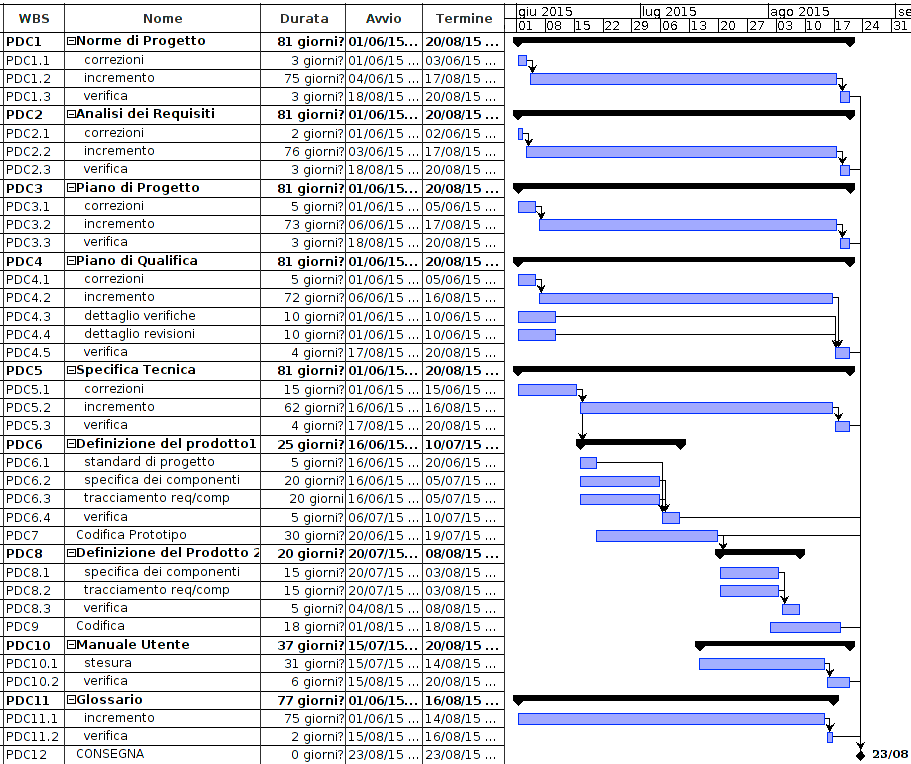
\includegraphics[width=\textwidth, height=\textheight, keepaspectratio]{img/progdet-gantt.png}
\caption{Diagramma di Gantt delle attività della macro-fase di Progettazione di Dettaglio e Codifica.}
\end{center}
\end{figure}
\clearpage

\newpage
\subsubsection{tabella persone/ore/attività}

\begin{figure}[h]
\begin{center}
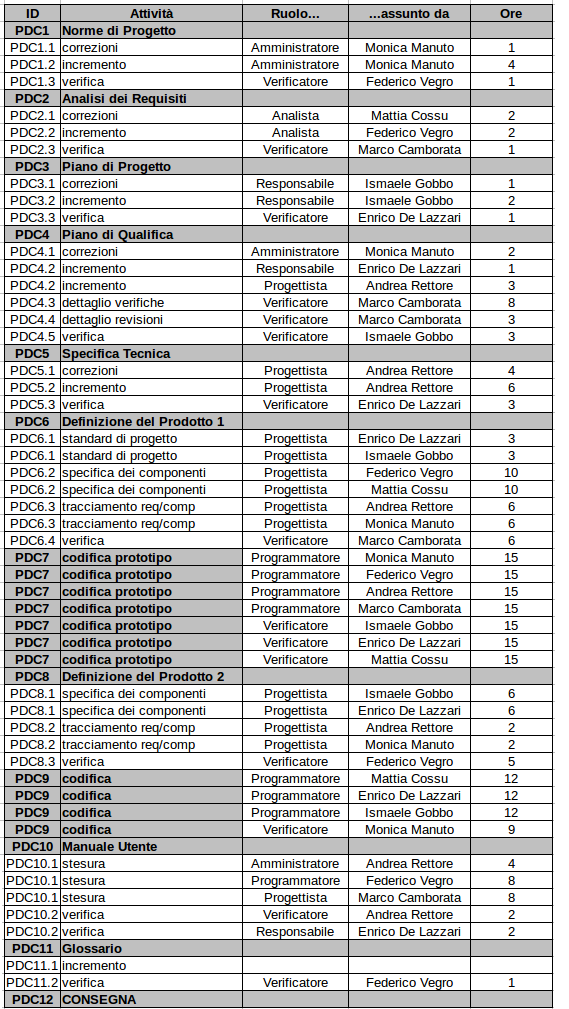
\includegraphics[scale=0.45]{img/progdet-attivita.png}
\caption{Tabella persone/ore/attività della macro-fase di Progettazione di Dettaglio e Codifica.}
\end{center}
\end{figure}
\clearpage

\subsubsection{tabella persone/ore/costi}

\begin{figure}[h]
\begin{center}
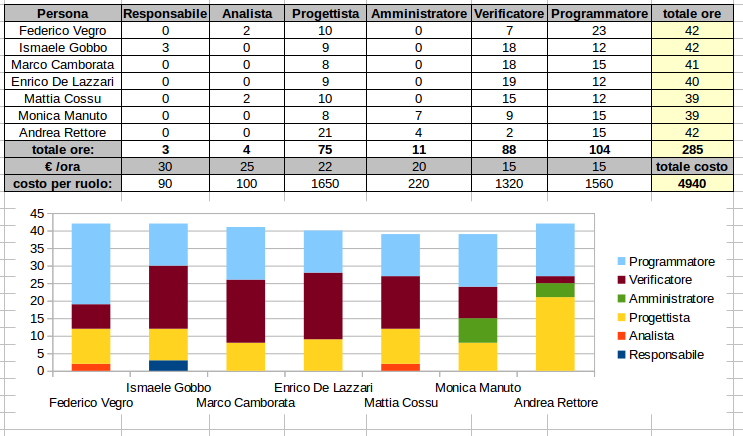
\includegraphics[scale=0.50]{img/progdet-personeorecosti.png}
\caption{Tabella persone/ore/costi della macro-fase di Progettazione di Dettaglio e Codifica.}
\end{center}
\end{figure}

\newpage
\subsection{Verifica Finale e Validazione}
\textbf{Periodo:} dal 2015-05-24 al 2015-06-16 \\
\textbf{Responsabile:} \CaMa \\
La macro-fase di Verifica Finale e Validazione inizia dalla Revisione di Qualifica e conclude le attività di sviluppo del software. \\
In queste tre settimane verrà corretta, incrementata e verificata tutta la documentazione prodotta fino a quel momento con l'obiettivo di rilasciarne una versione da definirsi completa. \\
L'attività di \textbf{validazione e collaudo} si occupa di accertare che il prodotto realizzato sia conforme alle attese e che copra i requisiti previsti. \\
I ruoli coinvolti sono quelli del \ruoloResponsabile{}, \ruoloAmministratore{}, \ruoloProgettista{}, \ruoloVerificatore{} e \ruoloProgrammatore{}. \\

\newpage
\subsubsection{diagramma di Gantt}

\begin{figure}[h]
\begin{center}
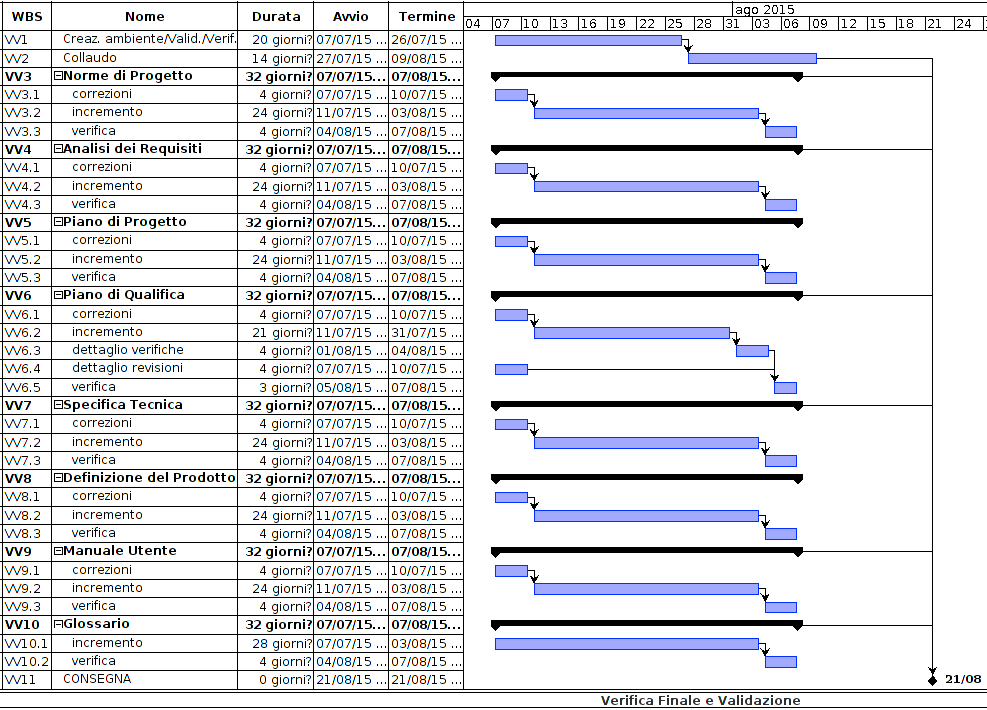
\includegraphics[width=\textwidth, height=\textheight, keepaspectratio]{img/verival-gantt.png}
\caption{Diagramma di Gantt delle attività della macro-fase di Verifica Finale e Validazione.}
\end{center}
\end{figure}
\clearpage

\newpage
\subsubsection{tabella persone/ore/attività}

\begin{figure}[h]
\begin{center}
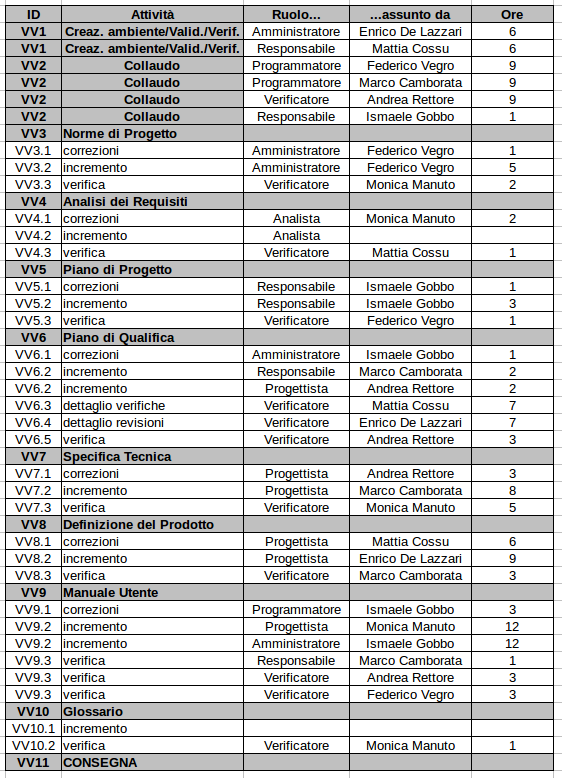
\includegraphics[scale=0.50]{img/verival-attivita.png}
\caption{Tabella persone/ore/attività della macro-fase di Verifica Finale e Validazione.}
\end{center}
\end{figure}
\clearpage

\subsubsection{tabella persone/ore/costi}

\begin{figure}[h]
\begin{center}
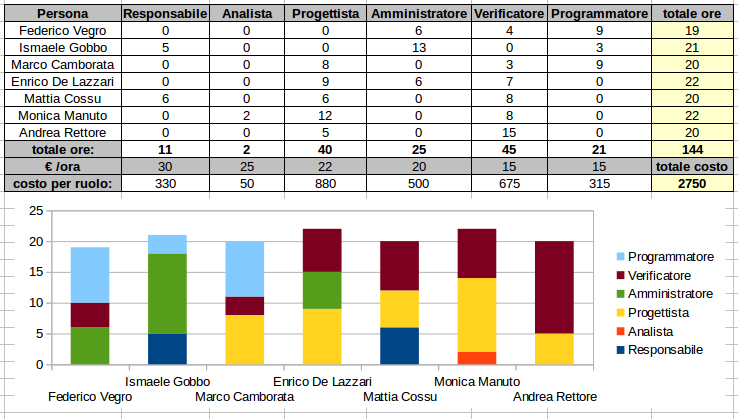
\includegraphics[scale=0.50]{img/verival-personeorecosti.png}
\caption{Tabella persone/ore/costi della macro-fase di Verifica Finale e Validazione.}
\end{center}
\end{figure}

\newpage

\section{Totale Costi e Ore}

\begin{figure}[h]
\begin{center}
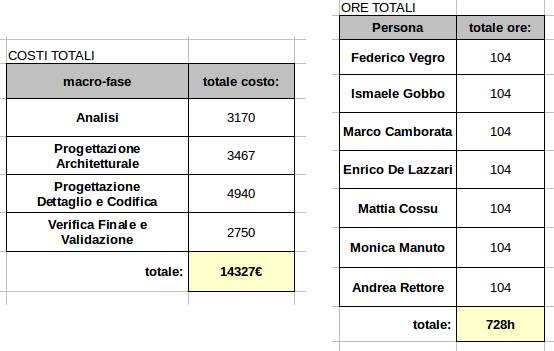
\includegraphics[scale=0.50]{img/totali.png}
\caption{Tabelle dei costi e delle ore totali.}
\end{center}
\end{figure}

Dalla sezione precedente si ricava un costo totale del progetto di \textbf{14327€}, e 104 ore complessive di lavoro per ciascun membro del gruppo.


